\documentclass{templateNote}
\usepackage{tcolorbox}
\usepackage{tabularx}
\usepackage{hyperref}
\usepackage{amsmath}
\usepackage{amssymb}
\usepackage{pdflscape}
\usepackage{tikz}
\usepackage{pdfpages}
\usepackage{soul}
\usepackage{media9}
\usepackage{adjustbox}
\usepackage{enumitem}
\usepackage{pdfpages}
\usepackage{mdframed} 
\usepackage{xcolor} 
% \usepackage[spanish,es-noquoting]{babel}

\begin{document}
% \linklogoU{https://www.ubiobio.cl/w/}
\linklogoD{https://github.com/NicoGomezM}
% \imagenlogoU{img/logo-ubb-txt-face.png}
\imagenlogoD{img/logoNGMFormal_sinF.png}
\titulo{Certamen 2}
\asignatura{Investigación de Operaciones}
\autor{
    Nicolás \textsc{Gómez Morgado}
}

\portada
\margenes
\tableofcontents
\newpage




\section{Materia}

\subsection{Cadenas de Markov}
\subsubsection{Proceso estocástico}
\noindent Es una sucesión $X_n$ de variables aleatorias, donde $n$ es un número entero no negativo. Se dice que $X_n$ es un proceso estocástico si para cada $n$, $X_n$ es una variable aleatoria.\\

\noindent\underline{\textbf{Ejemplo:}}

\noindent Supongamos que $X_n$ = Estado del clima en el dia $n$ = 1, 2, 3, ...\\ Supongamos que los estudios posibles son {n:nublado, s:soleado, r:lluvia}\\
\begin{center}
    $\Omega: {n,s,r}$ = Espacio muestral\\    
\end{center}

\noindent Realización de $X_n$:
\begin{center}
    $n,n,s,s,s,r,r,n,n,n;$
\end{center}

\noindent Supuestos para la cadena de Markov:
\begin{enumerate}
    \item El estado de la cadena en el instante $n+1$ depende solo del estado en el instante actual $n$ (no de anteriores[n-1,n-2,n-3...]).
    \item Con este supuesto se establecen las probabilidades condicionales homogéneas.\\
    $P_{ij}: $Probabilidad de pasar del estado i al estado j en una etapa. \\
    Notar que $P_{ij}$ no depende de $n$. \\
    Con esto se forma una matriz conformada por P = ($P_{ij})_{ij=1,2,3,...,*}$ \\
    P: Matriz de transición de probabilidades en una etapa.
    \item Supongamos que nuestros ejemplos:
    \begin{center}
        $P = $
        \[
        \begin{array}{l}
        \text{n} \\
        \text{s} \\
        \text{r} \\
        \end{array}
        \left(
        \begin{array}{ccc}
        0.7 & 0.2 & 0.1 \\
        0.1 & 0.6 & 0.3 \\
        0.2 & 0.3 & 0.5 \\
        \end{array}
        \right)
        \]
    \end{center}

    Obs.: Cada pila es una distribución de probabilidad condicional.\\

    \begin{align*}
        \sum_{j}^{} P_{ij} = 1 - P_i
    \end{align*}

    \newpage
    \item Para cada cadena de Markov P tiene asociados un dia de transición entre estados.\\
    \begin{figure}[H]
        \centering
        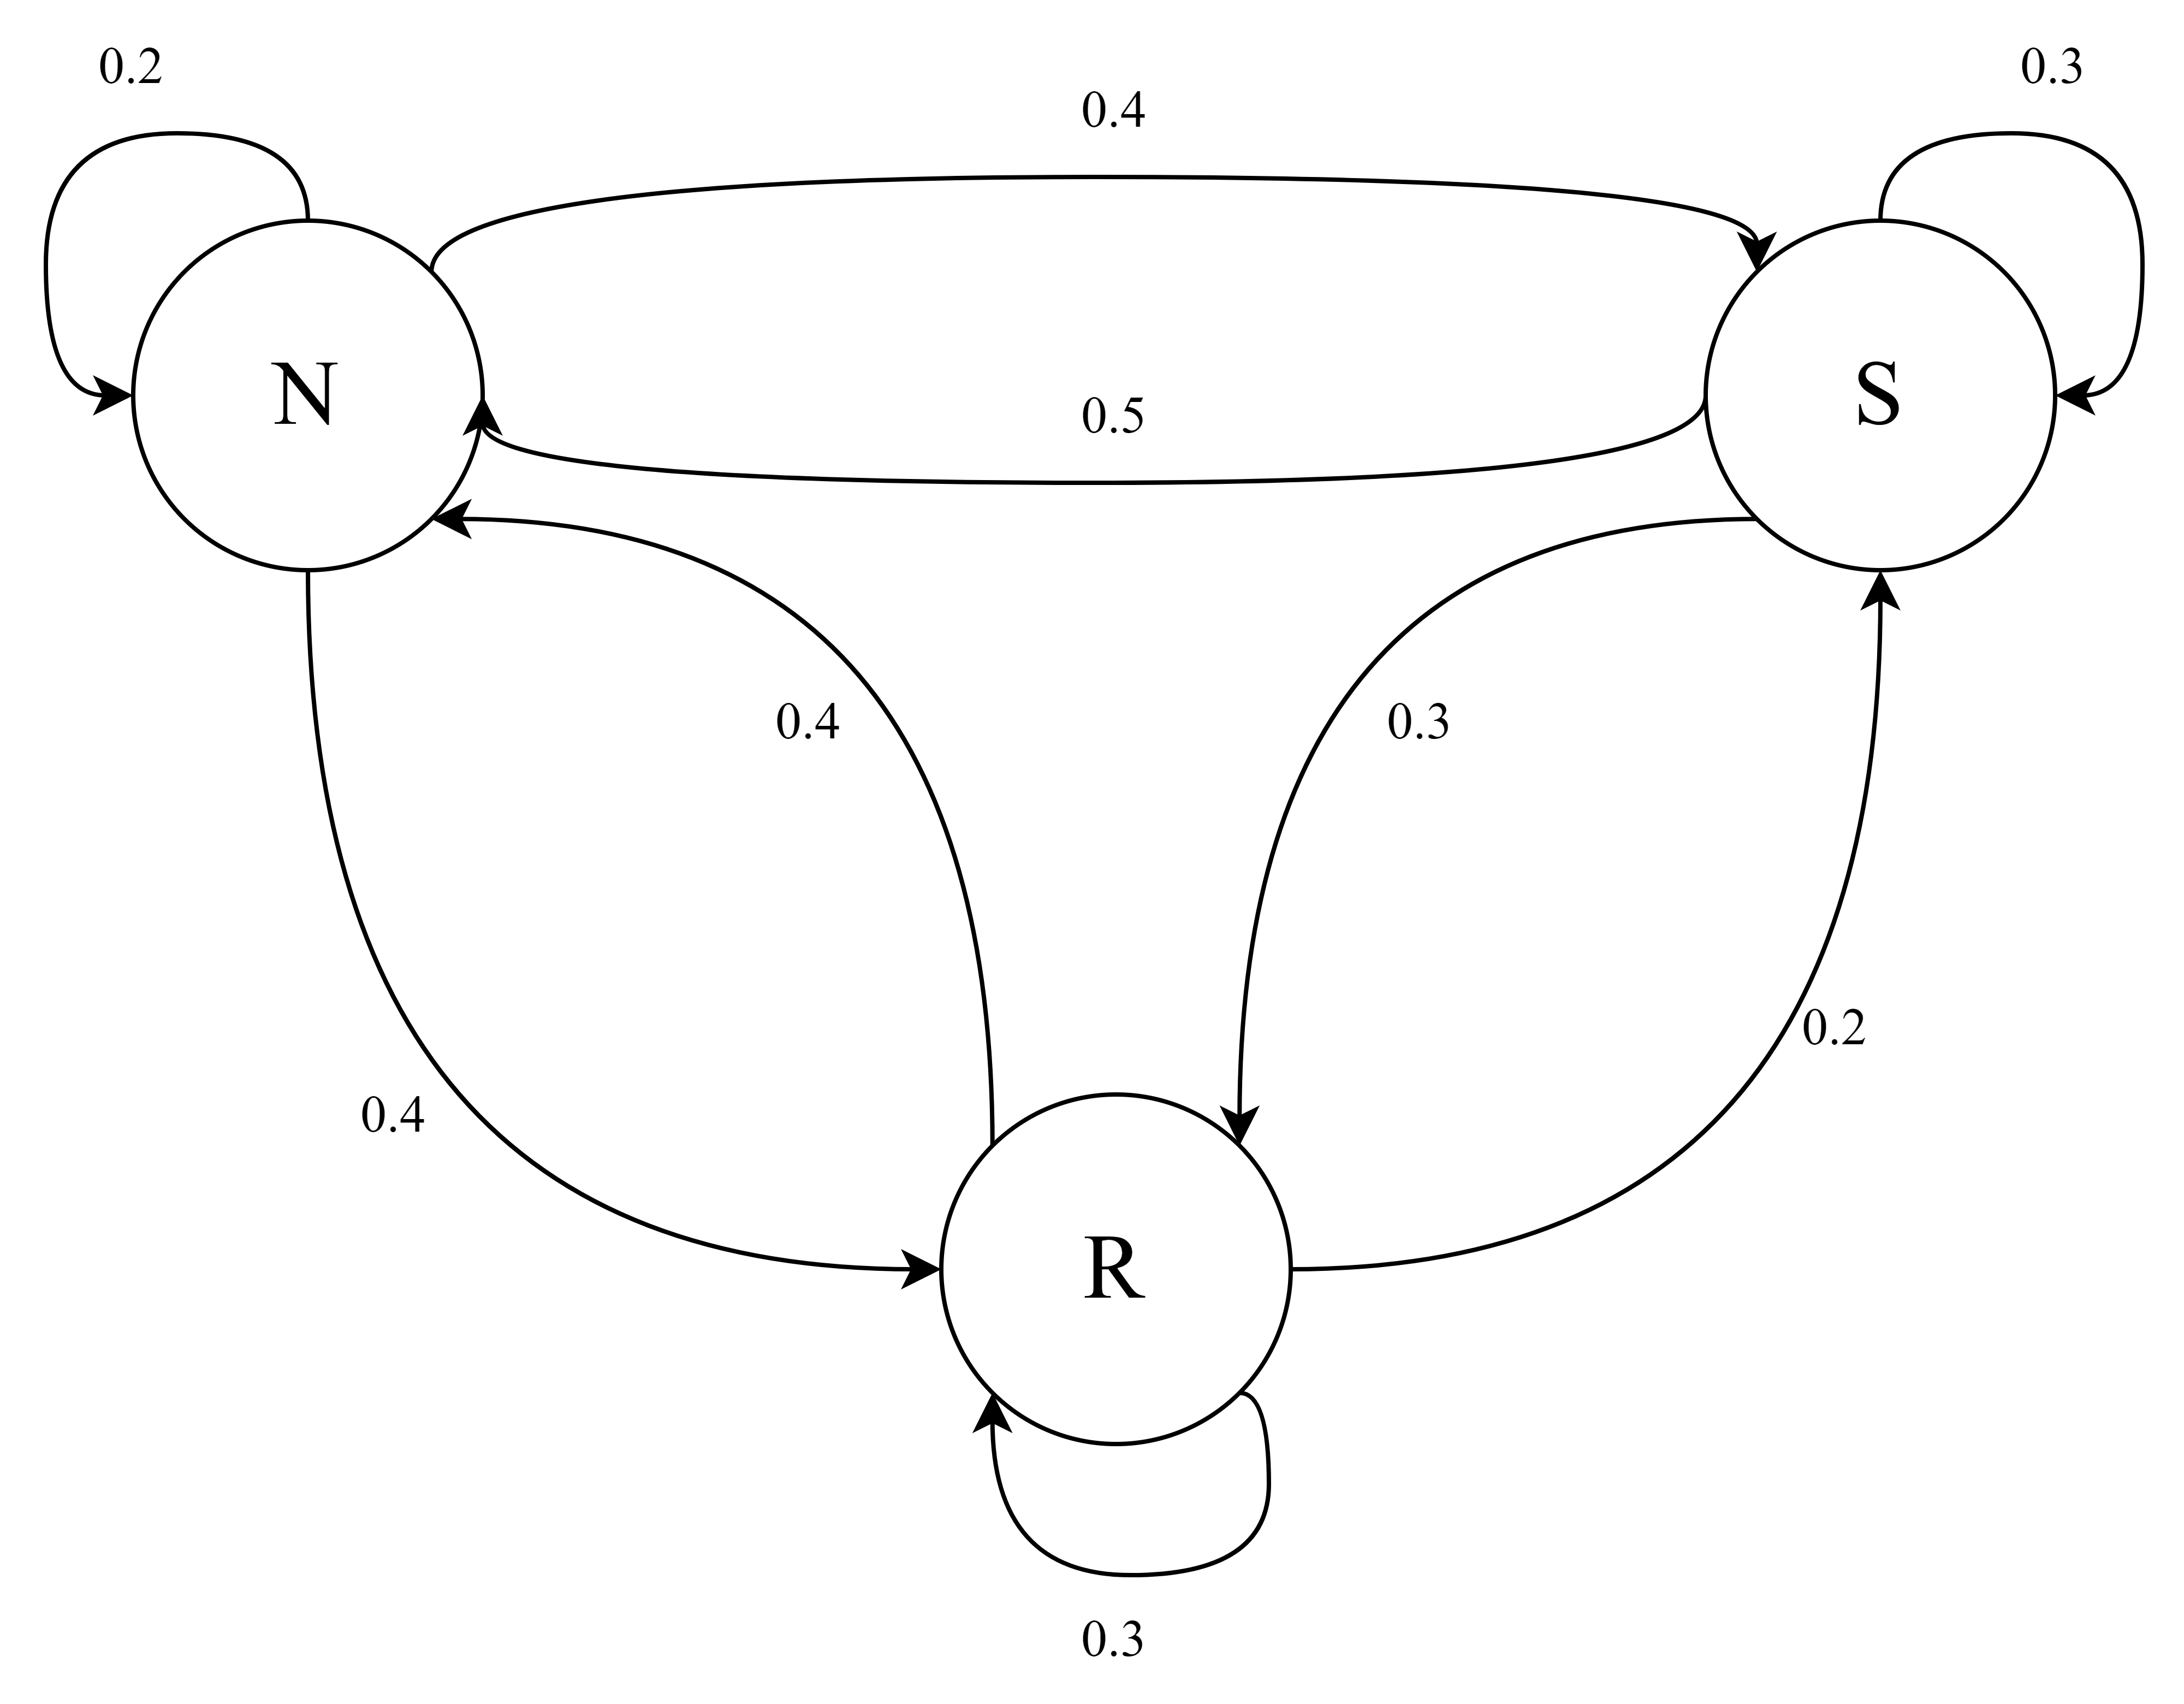
\includegraphics[width=0.8\textwidth]{img/estados.png}
    \end{figure}
\end{enumerate}


\end{document}